\documentclass[11pt]{article}
\usepackage{amsmath}
\usepackage{amssymb}
\usepackage{microtype}
\usepackage[english]{babel}
\usepackage[labelsep=period]{caption}
\usepackage[margin=4cm]{geometry}
\usepackage{graphicx}
\usepackage[utf8]{inputenc}
\usepackage{listings}
\usepackage{float}
\usepackage{xcolor}
\usepackage{subfigure}

\frenchspacing
\DisableLigatures[f]{}
\parindent=20pt

\definecolor{medgreen}{rgb}{0.0, 0.6, 0.0}
\definecolor{reddishmauve}{rgb}{0.6, 0.0, 0.3}
\lstset{language=Python, showstringspaces=false, numberfirstline=false, breaklines=true, numbers=left, stepnumber=1, tabsize=4,
basicstyle=\ttfamily, numberstyle=\tiny, commentstyle=\color{medgreen}\rmfamily, stringstyle=\color{reddishmauve}, keywordstyle=\color{blue}}

\DeclareMathOperator*{\argmin}{arg\,min}

\author{Ahmad Jamalzada \& Joseph Salaris}
\title{\textsc{\Huge Computational Physics}\\Molecular Dynamics}

\begin{document}
\maketitle

\section{Introduction}
Molecular systems consist of a large number of particles interacting with each other through some forces. It is impossible to analytically determine properties of these complex systems. To circumvent this problem we can use Molecular Dynamics (MD) simulations.
Molecular dynamics is a computer simulation method that uses numerical methods for studying many-particle systems such as molecules and macroscopic systems such as gases, liquids and solids.
As a first introduction to MD we will be simulating a system of Argon atoms. This is because argon atoms behave approximately like hard spheres which interact with each other through weak van der Waals forces. They also do not form any bonds and do not interact via Coulomb interaction, this simplifies the dynamics quite a bit.

Since we want to use a classical description of the argon system, we need to check if this is justified. We need to compare the inter-particle distance to de-Broglie wavelength. The typical distance between argon atoms is $\sim 5 \AA$.\cite{lattice} From statistical mechanics we know that the average kinetic energy of the argon atoms is $E_{kin} = \dfrac{p^2}{2m}=\dfrac{3}{2}k_BT$ and de-Broglie wavelength $\lambda=\dfrac{h}{p} \rightarrow \lambda = \dfrac{h}{\sqrt{3mk_bT}}$. For room temperature we arrive at $\lambda \approx 0.1 \AA \ll 5\AA$. So the motion of the atoms is classical.

The interaction between two argon atoms can be approximated quite well by a Lennard-Jones potential function:
\begin{align*}
U(r)=4\epsilon\Big[\Big(\dfrac{\sigma}{r}\Big)^{12}-\Big(\dfrac{\sigma}{r}\Big)^6\Big]
\end{align*}
where $r$ is the distance between the atoms, $\epsilon=1.65\times10^{-21}$J is the strength of the potential energy, and $\sigma = 3.4\times 10^{-10}$m is the value of $r$ at which the energy is zero. The $1/r^6$ force is due to the small displacement between the nucleus and the electron cloud which gives rise to a small dipole moment. This results in a attractive dipole-dipole (van der Waals) interaction. 
Since argon atoms do not form molecules, there needs to be a repulsive force that keeps them from overlapping, this is the $1/r^{12}$ repulsive force.

\begin{figure}[h!]
\centering
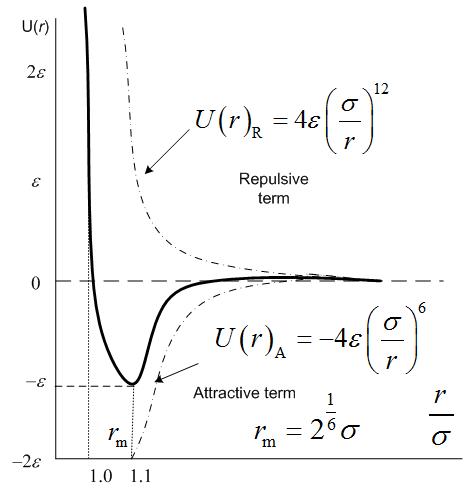
\includegraphics[width=0.6\textwidth]{lennard_jones}
\caption{Lennard-Jones potential. Figure obtained from \cite{lennard-jones}}\label{lj}
\end{figure}

In this report we will simulate a system of argon atoms in its gas, liquid and solid phase. To check if the MD simulation does indeed provide the behavior of the different phases, we can calculate the pair correlation function which characterizes the phase of the argon system. We will then calculate a few canonical averages for each phase.


\section{Methods}
In our simulation a system of $N=108$ particles in a box with sides of finite length $L$ is considered.  Periodic boundary conditions are imposed in order to simulate an infinite system of Argon atoms. For convenience and also to prevent round-off errors we work with 'reduced units' , where length is expressed in units of $\sigma$, energy in units of $\epsilon$, time in units of $\tau=(\frac{m\sigma^2}{\epsilon})^\frac{1}{2}=2.15\cdot10^{-12} s$ for Argon and temperature in units of $\epsilon/k_B=119.9 K$. 

As we describe the system classically the time-evolution is governed by Newton's equation of motion (in reduced units): 
\begin{align*}
 \frac{d^2\textbf{r$_i$}}{dt^2}=\sum_{j\ne i}\textbf{f}(r_{ij})
\end{align*}
where the force is determined by the Lennard-Jones potential. For the interaction distance $r_{ij}$  we use the minimum image convention,  i.e. the distance within the box or the distance w.r.t. the image particle introduced by the periodic boundary conditions, whichever is shorter. We integrate by using the velocity-Verlet algorithm \cite{vv-algorithm}:
\begin{align*}
&\textbf{r}(t+dt)=\textbf{r}(t)+\textbf{v(t)}dt+\frac{\textbf{f}}{2}dt^2\\
&\textbf{v}(t+dt)=\textbf{v(t)}+\frac{\textbf{f}(t+dt)+\textbf{f}(t)}{2}dt
\end{align*}
thus the particles evolve in finite timesteps, where the time increment is set to $dt=0.004$. With each timestep the $\frac{N(N-1)}{2}$ interaction distances are computed, subsequently the forces and finally the particles' positions and velocities are updated. 

The initial positions are set to a fcc lattice, which happens to be the ground state configuration for solid Argon. Moreover in this way we prevent the particles from being too close to each other, as otherwise  the $r^{-12}$ potential  increases significantly forcing one to use smaller time increment, thus limiting computation time. The initial velocities are chosen from a Gaussian distribution such that a Maxwell-Boltzmann distribution $e^{\frac{-mv^2}{k_bT}}$ is obtained with a given temperature. As the system equilibrates the temperature changes, hence in order to control the temperature of the system we rescale the velocities: 
\begin{align*}
\textbf{v}\longrightarrow\lambda\textbf{v}
\end{align*}
where from the equipartition theorem $E_{kin}=(N-1)\dfrac{3}{2}k_BT$ we find the rescaling factor: 
\begin{align*}
\lambda=\sqrt{\frac{(N-1)3k_BT}{\sum mv_i^2}}
\end{align*}
The factor of $(N-1)$ is due to the constraint of conservation of momentum reducing the degrees of freedom. 

In our simulation we run the system for $5000$ timesteps amounting to a simulation time of $20\tau$. The system is allowed to come to equilibrium for $500$ timesteps whereafter the system is rescaled for $2500$ timesteps with a cycle of $20$ timesteps. The remaining $2000$ timesteps forms the production phase, from which we compute canonical averages and the pair correlation function. Throughout the simulation we extract the instantaneous temperature (again using the equipartition theorem), the potential and kinetic energy as shown in figure \ref{methods}. The pair correlation function is made by creating a histogram of the number of pairs of particles $n(r)$ with a separation distance r. In terms of $n(r)$ the correlation function is given by:
\begin{align*}
g(r)=\frac{2V}{N(N-1)}\left[\frac{\langle n(r)\rangle}{4\pi r^2\triangle r}\right]
\end{align*}
where $\triangle r$ is the bin size and $V$ is the volume of the box.



\begin{figure}
\hfill
\subfigure[Energy]{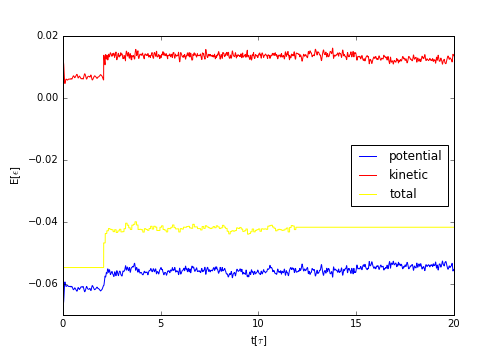
\includegraphics[width=0.49\textwidth]{energy_methods}}
\hfill
\subfigure[Temperature]{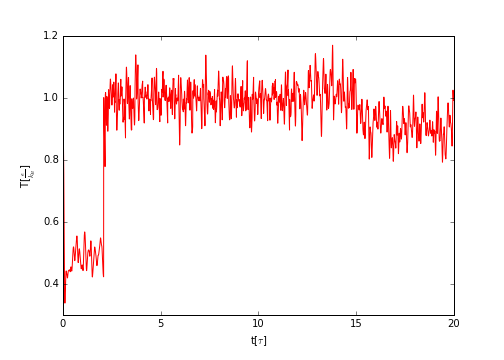
\includegraphics[width=0.49\textwidth]{temperature_methods}}
\hfill
\caption{The temperature kinetic, potential and total energy extracted throughout the simulation (equilibration, rescaling and production phase) are shown.}\label{methods}
\end{figure}


Errors in averages are calculated by bootstrapping the extracted data points and treating them as independent datasets, hence computing the average for each dataset. The error is then given by:
\begin{align*}
\sigma_A=\sqrt{\langle A^2\rangle-\langle A\rangle^2}
\end{align*}
For the propagation of errors we use the standard method:
\begin{align*}
\sigma_B=\sqrt{\left(\frac{dB}{dx}\right)^2\sigma_x^2+\left(\frac{dB}{dy}\right)^2\sigma_y^2}
\end{align*}
with $B$ a variable dependent on $x$ and $y$. 

As a reference we use \cite{book} to check our simulation. Setting the density $\rho=0.88 \frac{1}{\sigma^3}$ and $T_0=1.0\frac{\epsilon}{k_B}$  we find for the simulation temperature $T=0.954\pm2\cdot10^{-3}\frac{\epsilon}{k_B}$, the compressibility $Z=2.46\pm8\cdot10^{-2}$ and the potential energy per particle $U=-5.916\pm2\cdot10^{-3}\epsilon$. These values correspond reasonably well with \cite{book}.

\section{Results}
We present our results obtained from the production phase of our simulation of argon atoms. 
\begin{table}[h!]
\caption{Canonical averages temperature $T$, compressibility $Z$ and potential energy per particle $U$ corresponding to the three phases solid, liquid and gas found from the simulation of the argon system.}\label{ca}
\begin{tabular}{ccc|c|c|c}
$\text{phase}$&$\text{$\rho[1/\sigma^3]$}$&$\text{$T_0$[1/$\epsilon$]}$&$\text{T[1/$\epsilon$]}$&$\text{Z}$&$\text{U[$\epsilon$]}$\\\hline
solid&$1.2$&$0.5$&$0.5165\pm5\cdot10^{-4}$&$0.64\pm6\cdot10^{-2}$&$-5.952\cdot10^{-4}\pm6\cdot10^{-8}$\\
liquid&$0.8$&$1$&$0.969\pm1\cdot10^{-3}$&$1.04\pm2\cdot10^{-2}$&$-5.357\pm2\cdot10^{-3}$\\
gas&0.3&3.0&$3.045\pm2\cdot10^{-3}$&$1.01\pm1\cdot10^{-2}$&$-1.706\pm3\cdot10^{-3}$
\end{tabular}
\end{table}
Note that in table \ref{ca} that the temperature extracted from the simulation is not exactly equal to the input temperature as after rescaling it fluctuates around its equilibrium. As expected the compressibility is closest to one in the gas phase. Furthermore we observe that the potential energy is  larger for the solid phase than for liquid and gas phase. This could be because the conversion of potential energy to kinetic energy occurs less as the positions of the particles are more rigid.

\begin{figure}[h!]
\centering
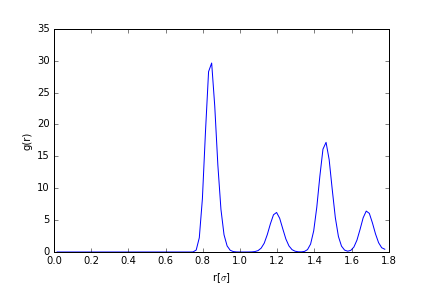
\includegraphics[width=0.7\textwidth]{correlation_solid}
\caption{Pair correlation function as obtained from the simulation of the system in the solid phase.}\label{solid}
\end{figure}

In figure \ref{solid} we denote sharp peaks of the correlation function of the system in the solid phase. In a solid, the distances between pairs of atoms is much more uniform which corresponds to the sharp peaks. Multiple peaks show that the system easily configure into equilibrium positions, where the first peak corresponds to initial positions which is the fcc lattice. 

\begin{figure}[h!]
\centering
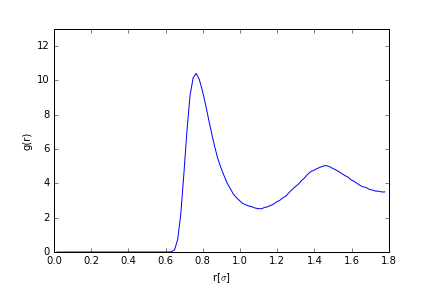
\includegraphics[width=0.7\textwidth]{correlation_liquid}
\caption{Pair correlation function as obtained from the simulation of the system in the liquid phase.}\label{liquid}
\end{figure}

In figure \ref{liquid} we see that the correlation function in the liquid phase is smooth, however remnants of the lattice configuration as found in the solid phase remain.

\begin{figure}[h!]
\centering
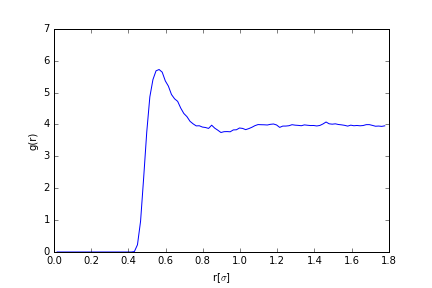
\includegraphics[width=0.7\textwidth]{correlation_gas}
\caption{Pair correlation function as obtained from the simulation of the system in the gas phase.}\label{gas}
\end{figure}

 In the gas phase, figure \ref{gas} we see only the peak corresponding to the initial positions and all larger separation distances are equally distributed which correponds to the broad velocity distribution of the particles.

%\newpage
\section{Conclusion}
We have shown that we can characterize different phases of an argon system using a Molucelar Dynamics (MD) simulation. Assuming the interaction is given by the Lennard-Jones potential and integrating the equations of motions via the velocity-Verlet algorithm we have obtained the pair correlation function. We found distinct behaviour of the pair correlation function for the three different phases. Furthermore we extracted some canonical averages.


\begin{thebibliography}{x}
\bibitem{lattice}
http://www.infoplease.com/periodictable.php?id=18
\bibitem{lennard-jones}
Carl Y. H. Jiang, A New Approach to Model Adsorption in Heterogeneous
Phase System with Monte Carlo Method, American Journal of Materials Science 2014, 4(1): 25-38
\bibitem{vv-algorithm}
Loup Verlet, Computer "Experiments" on Classical Fluids. I. Thermodynamical Properties of Lennard-Jones Molecules, Phys. Rev. 159, 98 (1967)
\bibitem{book}
Jos Thijssen, Computational Physics 2nd Edition, page 224
\end{thebibliography}


\end{document}
